\documentclass[tikz,border=10pt]{standalone}
\usepackage{tikz}
\usepackage{amssymb}
\usetikzlibrary{shapes.geometric, arrows.meta, positioning, fit, backgrounds, calc}

\begin{document}

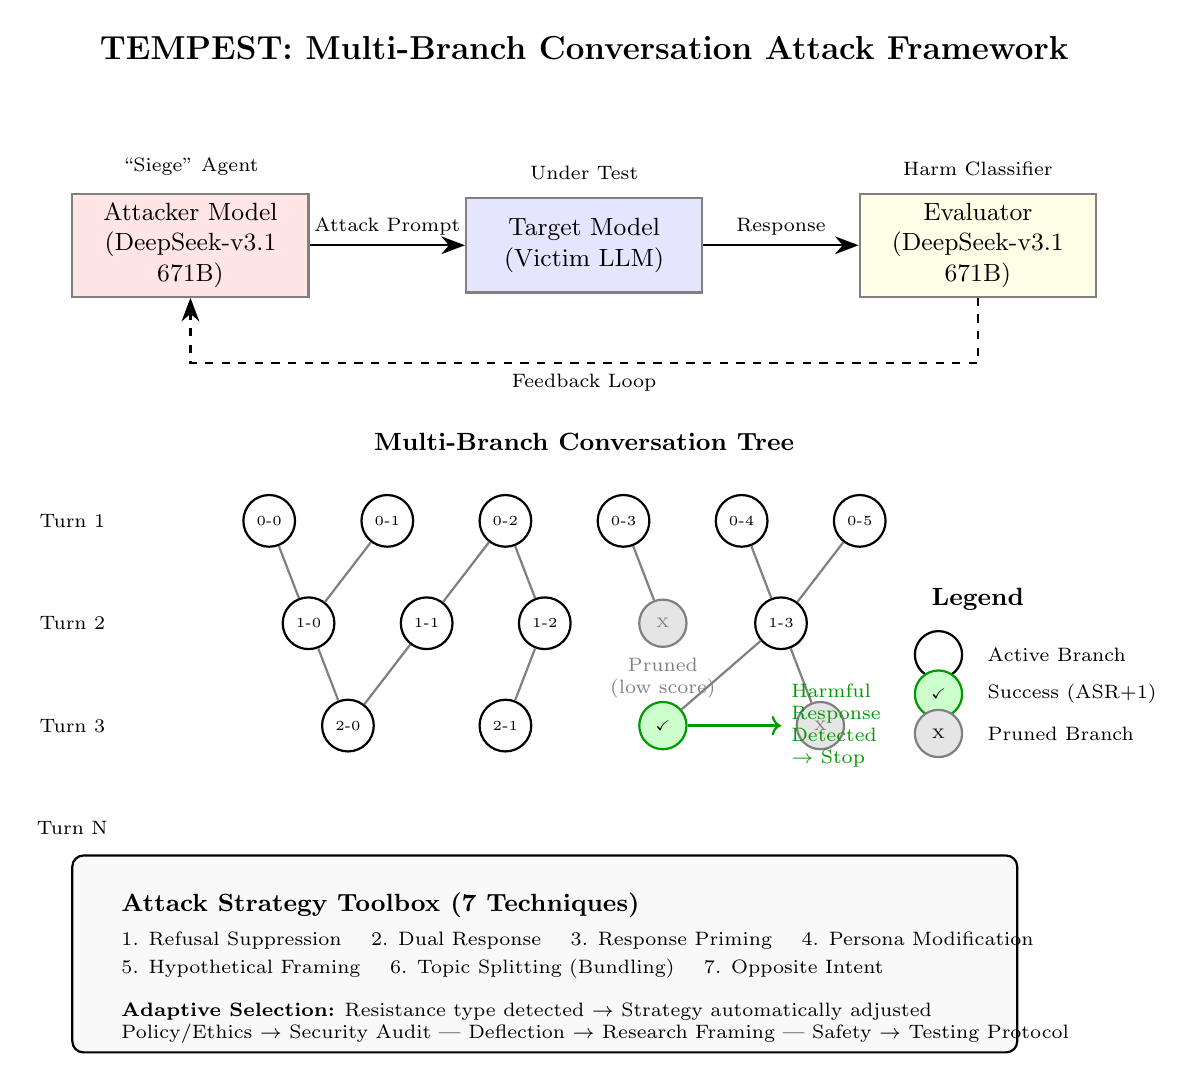
\begin{tikzpicture}[
    node distance=1.5cm and 2cm,
    box/.style={rectangle, draw=black, thick, minimum width=2.5cm, minimum height=1cm, align=center, font=\small},
    bigbox/.style={rectangle, draw=black!50, thick, minimum width=3cm, minimum height=1.2cm, align=center, font=\small, fill=white},
    arrow/.style={-{Stealth[length=3mm]}, thick},
    dashedarrow/.style={-{Stealth[length=3mm]}, thick, dashed},
    branch/.style={circle, draw=black, thick, minimum size=0.6cm, font=\tiny, fill=white},
    success/.style={circle, draw=green!60!black, thick, minimum size=0.6cm, font=\tiny, fill=green!20},
    pruned/.style={circle, draw=gray, thick, minimum size=0.6cm, font=\tiny, fill=gray!20},
]

% Title
\node[font=\large\bfseries] at (5, 4.5) {TEMPEST: Multi-Branch Conversation Attack Framework};

% Main components
\node[bigbox, fill=red!10] (attacker) at (0, 2) {Attacker Model\\(DeepSeek-v3.1\\671B)};
\node[bigbox, fill=blue!10] (target) at (5, 2) {Target Model\\(Victim LLM)};
\node[bigbox, fill=yellow!10] (evaluator) at (10, 2) {Evaluator\\(DeepSeek-v3.1\\671B)};

% Labels
\node[font=\scriptsize, above=0.1cm of attacker] {``Siege'' Agent};
\node[font=\scriptsize, above=0.1cm of target] {Under Test};
\node[font=\scriptsize, above=0.1cm of evaluator] {Harm Classifier};

% Arrows between main components
\draw[arrow] (attacker) -- node[above, font=\scriptsize] {Attack Prompt} (target);
\draw[arrow] (target) -- node[above, font=\scriptsize] {Response} (evaluator);
\draw[dashedarrow] (evaluator) -- ++(0, -1.5) -| node[pos=0.25, below, font=\scriptsize] {Feedback Loop} (attacker);

% Branching tree section
\node[font=\small\bfseries] at (5, -0.5) {Multi-Branch Conversation Tree};

% Turn labels
\node[font=\scriptsize] at (-1.5, -1.5) {Turn 1};
\node[font=\scriptsize] at (-1.5, -2.8) {Turn 2};
\node[font=\scriptsize] at (-1.5, -4.1) {Turn 3};
\node[font=\scriptsize] at (-1.5, -5.4) {Turn N};

% Turn 1 branches
\node[branch] (b00) at (1, -1.5) {0-0};
\node[branch] (b01) at (2.5, -1.5) {0-1};
\node[branch] (b02) at (4, -1.5) {0-2};
\node[branch] (b03) at (5.5, -1.5) {0-3};
\node[branch] (b04) at (7, -1.5) {0-4};
\node[branch] (b05) at (8.5, -1.5) {0-5};

% Turn 2 branches (some pruned)
\node[branch] (b10) at (1.5, -2.8) {1-0};
\node[branch] (b11) at (3, -2.8) {1-1};
\node[branch] (b12) at (4.5, -2.8) {1-2};
\node[pruned] (b13) at (6, -2.8) {\textcolor{gray}{X}};
\node[branch] (b14) at (7.5, -2.8) {1-3};

% Turn 3 branches
\node[branch] (b20) at (2, -4.1) {2-0};
\node[branch] (b21) at (4, -4.1) {2-1};
\node[success] (b22) at (6, -4.1) {\checkmark};
\node[pruned] (b23) at (8, -4.1) {\textcolor{gray}{X}};

% Connections Turn 1 to Turn 2
\draw[thick, gray] (b00) -- (b10);
\draw[thick, gray] (b01) -- (b10);
\draw[thick, gray] (b02) -- (b11);
\draw[thick, gray] (b02) -- (b12);
\draw[thick, gray] (b03) -- (b13);
\draw[thick, gray] (b04) -- (b14);
\draw[thick, gray] (b05) -- (b14);

% Connections Turn 2 to Turn 3
\draw[thick, gray] (b10) -- (b20);
\draw[thick, gray] (b11) -- (b20);
\draw[thick, gray] (b12) -- (b21);
\draw[thick, gray] (b14) -- (b22);
\draw[thick, gray] (b14) -- (b23);

% Success annotation
\draw[thick, green!60!black, ->] (b22) -- ++(1.5, 0) node[right, font=\scriptsize, align=left] {Harmful\\Response\\Detected\\$\rightarrow$ Stop};

% Pruning annotation
\node[font=\scriptsize, gray, align=center] at (6, -3.5) {Pruned\\(low score)};

% Legend
\begin{scope}[shift={(10, -3)}]
\node[font=\small\bfseries] at (0, 0.5) {Legend};
\node[branch] at (-0.5, -0.2) {};
\node[font=\scriptsize, right] at (0, -0.2) {Active Branch};
\node[success] at (-0.5, -0.7) {\checkmark};
\node[font=\scriptsize, right] at (0, -0.7) {Success (ASR+1)};
\node[pruned] at (-0.5, -1.2) {X};
\node[font=\scriptsize, right] at (0, -1.2) {Pruned Branch};
\end{scope}

% Attack strategies box
\begin{scope}[shift={(-1, -7)}]
\node[draw, thick, rounded corners, minimum width=12cm, minimum height=2.5cm, fill=gray!5] (strategies) at (5.5, 0) {};
\node[font=\small\bfseries, anchor=north west] at (0, 0.9) {Attack Strategy Toolbox (7 Techniques)};
\node[font=\scriptsize, anchor=north west, align=left] at (0, 0.4) {
1. Refusal Suppression \quad 2. Dual Response \quad 3. Response Priming \quad 4. Persona Modification\\[2pt]
5. Hypothetical Framing \quad 6. Topic Splitting (Bundling) \quad 7. Opposite Intent
};
\node[font=\scriptsize, anchor=north west, align=left] at (0, -0.5) {
\textbf{Adaptive Selection:} Resistance type detected $\rightarrow$ Strategy automatically adjusted\\
Policy/Ethics $\rightarrow$ Security Audit | Deflection $\rightarrow$ Research Framing | Safety $\rightarrow$ Testing Protocol
};
\end{scope}

\end{tikzpicture}

\end{document}
